%-----------------------circuit 1--------------------------
\section{Single Phase Half Wave Uncontrolled Rectifier with R load}

\subsection{Circuit used for simulation}

% figure that is centered on the page
\begin{figure}[h]
    \centering
    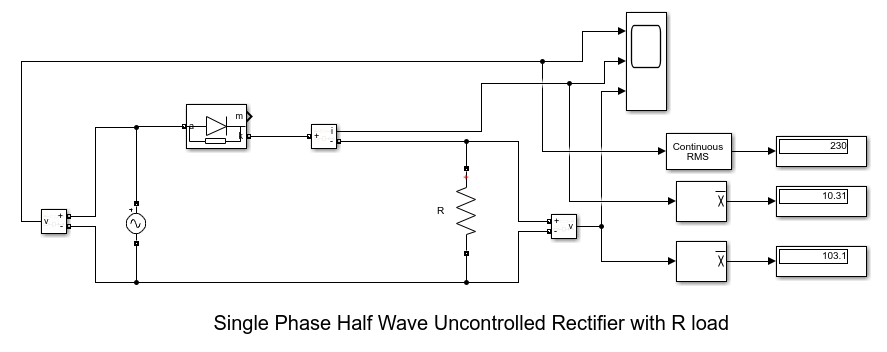
\includegraphics[width=0.7\textwidth]{images/experiment-1/circuit-diagram-simulation-01.png}
    \caption{Circuit used for simulation}
    \label{Fig_simulation_circuit_single-phase-half-wave-uncontrolled-rectifier-with-R-load}
\end{figure}

\subsection{Components Required}

\begin{table}[h]
    \renewcommand{\arraystretch}{1.3}
    \label{table_components_required_circuit_1}
    \centering
    \begin{tabular}{|c|c|c|c|}
        \hline
        Sr. No & Parameters                     & Ratings            & Quantity \\
        \hline
        \hline
        1      & AC Single Phase Voltage Source & 230V ($ V_{rms} $) & 1        \\
        \hline
        2      & Resistor                       & 10$ \Omega $       & 1        \\
        \hline
        3      & Diode                          & -                  & 1        \\
        \hline
        4      & Voltmeter                      & -                  & 2        \\
        \hline
        5      & Ammeter                        & -                  & 1        \\
        \hline
    \end{tabular}
    \caption{Components for Single Phase Half Wave Uncontrolled Rectifier with R load}

\end{table}




\subsection{Observations}

\begin{table}[h]
    \renewcommand{\arraystretch}{1.3}
    \label{table_observation_circuit_1}
    \centering
    \begin{tabular}{|c|c|c|}
        \hline
        Parameters                              & Theoretical Values & Simulation Values \\
        \hline
        \hline
        AC Input Voltage ($ V_{in,rms} $)       & 230V               & 230V              \\
        \hline
        Output Average Voltage ($ V_{o,avg} $)  & 103.53V            & 103.1V            \\
        \hline
        Output Average Current ($ I_{o,avg}  $) & 10.35A             & 10.31A            \\
        \hline
        AC Input Power ($ P_{AC}  $)            & 2389.5 W           & 2636 W            \\
        \hline
        DC Input Power ($ P_{DC}  $)            & 1071.53 W          & 1063 W            \\
        \hline
        Efficiency (\%)                         & 44.84              & 40.34             \\
        \hline
    \end{tabular}
    \caption{Observations for Single Phase Half Wave Uncontrolled Rectifier with R load}

\end{table}


Upon observation, it is discerned that the simulated values coincide precisely with the corresponding theoretical values. Owing to the resistive nature of the load, the output current is in phase with the output voltage. Analysis of the output voltage and current waveforms reveals that the diode conducts during the positive half-cycle of the AC source, while it becomes reverse-biased during the negative half-cycle.

\pagebreak

\subsection{Resultant Waveforms}

% figure that is centered on the page
\begin{figure}[h]
    \centering
    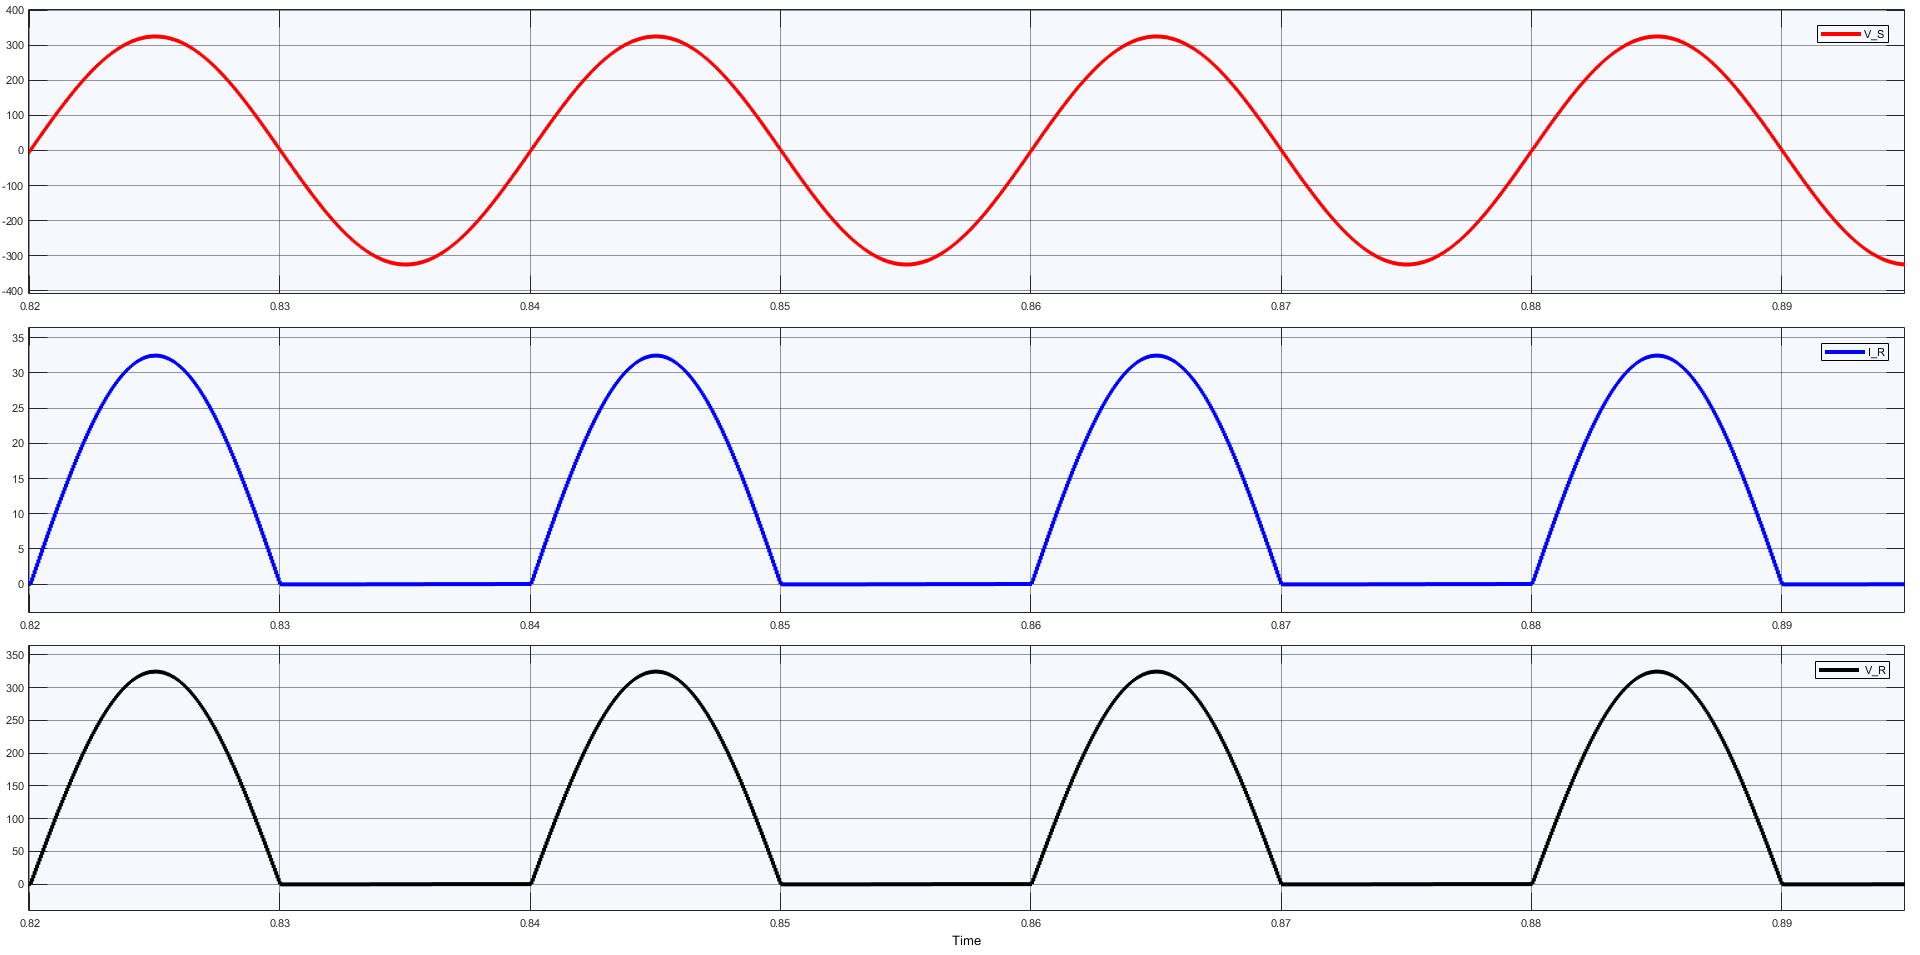
\includegraphics[width=1\textwidth]{images/experiment-1/circuit-scope-simulation-01.png}
    \caption{Scope Waveforms for Single Phase Half Wave Uncontrolled Rectifier with R load waveforms}
    \label{Fig_waveform_single-phase-half-wave-uncontrolled-rectifier-with-R-load}
\end{figure}

\pagebreak
